\newpage
\section*{Anexo 1}\label{Anx1}
\renewcommand{\theequation}{A\textsubscript{1}.\arabic{equation}}

En este primer anexo vamos a deducir el volumen de una hiperesfera de radio $R$ de dimensión $n$, de ecuación
\begin{equation}
	x_1^2+x_2^2 + \cdots + x_n^2 = R^n
\end{equation}
En general, sabemos que será proporcional a su radio de la forma
\begin{equation}
	V_n = C_nR^n
\end{equation}
donde $C_n$ es una constante que debemos determinar.
Para ello comenzamos con la definición de la superficie, que no será más que la derivada del volumen
\begin{equation}
	dS_n(R) = C_n n R^{n-1} dR
\end{equation}

\begin{align}
	\int_{-\infty}^{\infty} \dd{x_1} \int_{-\infty}^{\infty} \dd{x_2} \cdots \int_{-\infty}^{\infty} \dd{x_n}e^{-(x_1^2+x_2^2 + \cdots + x_n^2)} &= \int_{0}^{\infty} \dd{S_n} e^{-R^2} \nonumber \\
	\int_{-\infty}^{\infty} \dd{x_1} e^{-x_1^2} \int_{-\infty}^{\infty} \dd{x_2} e^{-x_2^2} \cdots \int_{-\infty}^{\infty} \dd{x_n} e^{-x_n^2} &= \int_{0}^{\infty} \dd{R} C_n n R^{n-1} e^{-R^2} \\
	\left[ 2 \int_{0}^{\infty} \dd{x_1} e^{-x_1^2} \right]^N &=  C_n n \int_{0}^{\infty} \dd{R} R^{n-1} e^{-R^2}\nonumber
\end{align}

Evaluemos ambos miembros por separado.
Para la integral del lado izquierdo realizamos el cambio de variable $x^2=t$
\begin{equation}
	2 \int_{0}^{\infty} \dd{x} e^{-x^2} = 2\frac{1}{2} \int_{0}^{\infty} \dd{t} t^{1/2} e^{-t} = \Gamma\left(\frac{1}{2}\right) = \sqrt{\pi}
\end{equation}
y para la del derecho, $R^2 = t$
\begin{equation}
	C_n n \int_{0}^{\infty} \dd{R} R^{n-1} e^{-R^2} = C_n n \frac{1}{2} \int_{0}^{\infty} \dd{t} t^{n - 1/2} e^{-t} = C_n \frac{n}{2} \Gamma\left(\frac{n}{2}\right)
\end{equation}
y recomponiendo
\begin{equation}
	\pi^{n/2} = C_n \frac{n}{2} \Gamma\left(\frac{n}{2}\right) \Rightarrow C_n = \pi^{n/2}\frac{2}{n}\frac{1}{\Gamma\left(\frac{n}{2}\right)} = \frac{\pi^{n/2}}{\Gamma\left(\frac{n}{2} + 1 \right)}
\end{equation}

Con lo que finalizamos con
\begin{equation}
	V_n = \frac{\pi^{n/2}}{\Gamma\left(\frac{n}{2} + 1 \right)}R^n
\end{equation}

\newpage
\section*{Anexo 2}\label{Anx2}
\renewcommand{\theequation}{A\textsubscript{2}.\arabic{equation}}
\setcounter{equation}{0}

En el anexo 2 vamos a desarrollar la \emph{fórmula de Stirling}, una aproximación válida para números muy grandes que es usada en varias ocasiones en el desarrollo de este documento.

La fórmula de Stirling comienza su desarrollo en la definición del factorial
\begin{equation}
	N! = N\cdot (N-1) \cdots 2 \cdot 1
\end{equation}
y, por tanto,
\begin{equation}
	\ln N! = \ln N + \cdots + \ln 1 = \sum_{n=1}^{N} \ln n
\end{equation}

\begin{wrapfigure}{r}{0.25\textwidth}
	\centering
	\hspace{2.5cm}
	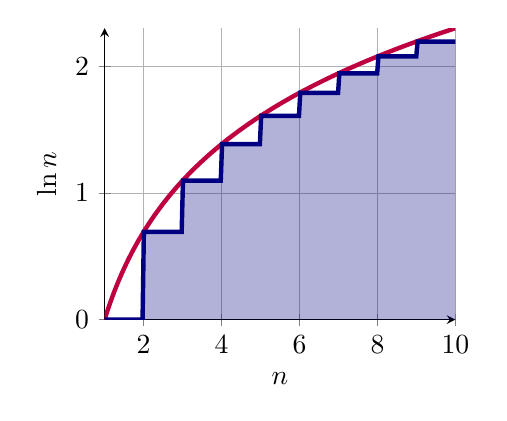
\begin{tikzpicture}
	\begin{axis}[
	scale = 0.65,
	samples=300,
	xmin = 1, xmax = 10,
	ymin = 0,
	axis lines=left,
	xlabel={$n$},
	ylabel={$\ln n$},
	xmajorgrids,
	x grid style={white!70!black},
	ymajorgrids,
	y grid style={white!70!black}]
	
	\addplot[purple, ultra thick, domain=0:10] {ln(x)};
	\addplot[NavyBlue, ultra thick, domain=0:10] {ln(floor(x))};
	
	\addplot [fill=NavyBlue, opacity=0.3, draw=none,domain=0:10] {ln(floor(x))} \closedcycle;
	
	\end{axis}
	\end{tikzpicture}
	\vspace{-0.5cm}
\end{wrapfigure}

Esta suma es igual al área encerrada por la línea poligonal de la figura entre $n = 1$ y $n = N$ (área sombreada).
Consideremos ahora el área encerrada entre los mismos valores de $n$ por la curva $y = \ln n$, también representada en la figura (línea sólida).
Para valores pequeños de $N$ ambas áreas difieren apreciablemente, pero al ir creciendo $N$ las dos curvas tienden a superponerse y las áreas encerradas por cada una de ellas se aproximan entre sí cada vez más.
No olvidemos que deseamos que sea pequeño el error relativo cometido al sustituir un área por otra y no su diferencia absoluta.
Recordando que el área encerrada entre una curva y el eje de abscisas viene dada por la integral definida, podemos escribir para valores grandes de $N$
\begin{equation}
	\ln N! \approx \int_{1}^{N} dn\ln n = \left[ n\ln n - n \right]_1^N
\end{equation}
o, despreciando la unidad frente a N,
\begin{equation}\label{eq:Stirl}
	\boxed{\ln N! \approx N\ln N - N}
\end{equation}
que es la fórmula de Stirling.

Desde luego existen expresiones más exactas, como la que podemos obtener a partir de la función $\Gamma$. Por definición
\begin{equation}
	n! = \int_0^\infty x^n e^{-x}\, dx
\end{equation}
que con el cambio de variable $x = ny$ y agrupando obtenemos
\begin{equation}
	n! = \int_0^\infty e^{n\ln x-x}\, dx = e^{n \ln n} n \int_0^\infty e^{n(\ln y -y)}\, dy
\end{equation}
y aplicando el método de Laplace obtenemos
\begin{equation}
	\int_0^\infty e^{n(\ln y -y)}\, dy \sim  \sqrt{\frac{2\pi}{n}} e^{-n}
\end{equation}
con lo que se obtiene la fórmula de Stirling
$$n! \approx \sqrt{2 \pi n} \; \left(\frac{n}{e}\right)^{n}$$

La expresión obtenida es una mera aproximación usando un orden bajo del método.
La expresión completa recibe el nombre de \emph{serie de Stirling}
\begin{equation}
	n! = \sqrt{2 \pi n} \; \left(\frac{n}{e}\right)^{n} \exp\left[ 
		{\frac{1}{12n}}
		-{\frac{1}{360n^3}}
		+{\frac{1}{1260n^5}}
		-{\frac{1}{1680n^7}}
		+\cdots \right] 
\end{equation}

Desarrollando dicha exponencial también se puede reescribir la fórmula como
\begin{equation}
	n! = \sqrt{2 \pi n} \; \left(\frac{n}{e}\right)^{n}
		\left(
			1
			+{\frac{1}{12n}}
			+{\frac{1}{288n^2}}
			-{\frac{139}{51840n^3n}}
			-{\frac{571}{2488320n^4}}
			+ \cdots
		\right)
\end{equation}
\begin{wrapfigure}{l}{0.4\textwidth}
	\centering
	\hspace{-1.5cm}
	% This file was created by matplotlib2tikz v0.6.15.
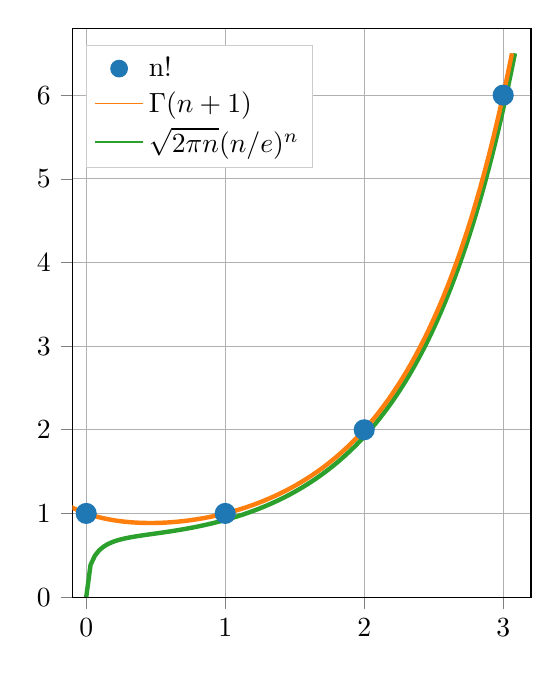
\begin{tikzpicture}
\definecolor{color0}{rgb}{0.12156862745098,0.466666666666667,0.705882352941177}
\definecolor{color1}{rgb}{1,0.498039215686275,0.0549019607843137}
\definecolor{color2}{rgb}{0.172549019607843,0.627450980392157,0.172549019607843}

\begin{axis}[
scale = 0.85,
xmin=-0.1, xmax=3.2,
ymin=0, ymax=6.8,
y = 1.25cm,
tick align=outside,
tick pos=left,
xmajorgrids,
ytick={0, 1, 2, 3, 4, 5, 6},
x grid style={white!69.01960784313725!black},
ymajorgrids,
y grid style={white!69.01960784313725!black},
legend cell align={left},
legend entries={{n!},{$\Gamma(n+1)$},{$\sqrt{2\pi n}(n/e)^n$}},
legend style={at={(0.03,0.97)}, anchor=north west, draw=white!80.0!black}
]
\addlegendimage{only marks, mark=*, mark size=3, mark options={solid}, color0}
\addlegendimage{no markers, color1}
\addlegendimage{no markers, color2}
\addplot [ultra thick, color2]
table {%
0 0
0.0311551563539123 0.384937373613077
0.0623103127078247 0.494535561784619
0.093465469061737 0.559262142698111
0.124620625415649 0.602635481943539
0.155775781769562 0.633721422320621
0.186930938123474 0.657055617672748
0.218086094477386 0.675233984886832
0.249241250831299 0.689872113596591
0.280396407185211 0.702035254008984
0.311551563539123 0.712456308427749
0.342706719893036 0.721656393607462
0.373861876246948 0.730015994308697
0.40501703260086 0.737819129829469
0.436172188954773 0.745281898420448
0.467327345308685 0.752571545394972
0.498482501662597 0.759819557422599
0.52963765801651 0.767130867644206
0.560792814370422 0.774590458546594
0.591947970724334 0.782268182259388
0.623103127078247 0.790222334587661
0.654258283432159 0.798502342047535
0.685413439786071 0.807150807607951
0.716568596139984 0.816205086292017
0.747723752493896 0.825698511835393
0.778878908847808 0.835661361501657
0.810034065201721 0.846121622492807
0.841189221555633 0.857105606725176
0.872344377909545 0.868638448839339
0.903499534263458 0.88074451370798
0.93465469061737 0.893447733414097
0.965809846971282 0.906771889023421
0.996965003325195 0.920740849007603
1.02812015967911 0.935378773565599
1.05927531603302 0.950710292111525
1.09043047238693 0.966760659684805
1.12158562874084 0.983555896874775
1.15274078509476 1.00112291695112
1.18389594144867 1.01948964319033
1.21505109780258 1.0386851188399
1.24620625415649 1.05873961173103
1.27736141051041 1.07968471521098
1.30851656686432 1.10155344679789
1.33967172321823 1.12438034574783
1.37082687957214 1.14820157055603
1.40198203592606 1.17305499728042
1.43313719227997 1.19898031947073
1.46429234863388 1.22601915040361
1.49544750498779 1.25421512825991
1.5266026613417 1.2836140248313
1.55775781769562 1.31426385830583
1.58891297404953 1.34621501065564
1.62006813040344 1.3795203501317
1.65122328675735 1.41423535935907
1.68237844311127 1.45041826952166
1.71353359946518 1.48813020112585
1.74468875581909 1.52743531183706
1.775843912173 1.56840095189337
1.80699906852692 1.61109782761274
1.83815422488083 1.65560017352739
1.86930938123474 1.70198593369835
1.90046453758865 1.75033695278654
1.93161969394256 1.80073917748209
1.96277485029648 1.85328286892278
1.99393000665039 1.90806282676392
2.0250851630043 1.96517862559661
2.05624031935821 2.02473486444871
2.08739547571213 2.08684143014333
2.11855063206604 2.1516137753331
2.14970578841995 2.21917321207523
2.18086094477386 2.28964722186234
2.21201610112778 2.36316978307736
2.24317125748169 2.43988171689816
2.2743264138356 2.51993105273819
2.30548157018951 2.60347341437442
2.33663672654342 2.6906724279832
2.36779188289734 2.7817001533781
2.39894703925125 2.87673753982238
2.43010219560516 2.97597490787237
2.46125735195907 3.07961245879659
2.49241250831299 3.18786081321044
2.5235676646669 3.30094158066666
2.55472282102081 3.41908796204903
2.58587797737472 3.54254538673074
2.61703313372864 3.67157218658005
2.64818829008255 3.80644030902516
2.67934344643646 3.94743607152728
2.71049860279037 4.09486095995737
2.74165375914429 4.24903247352732
2.7728089154982 4.41028501909212
2.80396407185211 4.57897085781585
2.83511922820602 4.75546110738176
2.86627438455993 4.94014680312689
2.89742954091385 5.13344002169385
2.92858469726776 5.33577507101944
2.95973985362167 5.54760975072049
2.99089500997558 5.76942668719472
3.0220501663295 6.00173474802735
3.05320532268341 6.24507054058641
3.08436047903732 6.49999999999955
};
\addplot [ultra thick, color1]
table {%
-0.2 1.1642297137253
-0.167037649753208 1.12916026205829
-0.134075299506415 1.09772343912734
-0.101112949259623 1.06952821057738
-0.0681505990128309 1.044241236184
-0.0351882487660386 1.02157696969694
-0.00222589851924637 1.00128973392686
0.0307364517275459 0.983167327956818
0.0636988019743382 0.967025833361151
0.0966611522211305 0.952705366539138
0.129623502467923 0.94006658341285
0.162585852714715 0.928987786775995
0.195548202961507 0.919362519680909
0.2285105532083 0.911097553349791
0.261472903455092 0.904111197285956
0.294435253701884 0.898331874047231
0.327397603948676 0.89369691262089
0.360359954195469 0.89015152331036
0.393322304442261 0.887647924101847
0.426284654689053 0.886144594066693
0.459247004935846 0.885605633805239
0.492209355182638 0.886000216501927
0.52517170542943 0.887302116031165
0.558134055676222 0.889489300876218
0.591096405923015 0.892543584512719
0.624058756169807 0.896450324452455
0.657021106416599 0.901198163410824
0.689983456663391 0.906778807106792
0.722945806910184 0.913186834070101
0.755908157156976 0.920419533550674
0.788870507403768 0.928476768226662
0.821832857650561 0.937360858912055
0.854795207897353 0.94707648888949
0.887757558144145 0.957630625853103
0.920719908390937 0.969032459751106
0.95368225863773 0.981293355077833
0.986644608884522 0.994426816387561
1.01960695913131 1.00844846599398
1.05256930937811 1.02337603298472
1.0855316596249 1.03922935282415
1.11849400987169 1.05603037694334
1.15145636011848 1.07380319182641
1.18441871036528 1.09257404720009
1.21738106061207 1.11237139302019
1.25034341085886 1.13322592502647
1.28330576110565 1.155170638708
1.31626811135244 1.17824089158486
1.34923046159924 1.20247447377132
1.38219281184603 1.22791168684013
1.41515516209282 1.25459543105885
1.44811751233961 1.28257130111765
1.48107986258641 1.31188769051425
1.5140422128332 1.34259590480654
1.54700456307999 1.37475028398673
1.57996691332678 1.40840833427413
1.61292926357358 1.44363086966559
1.64589161382037 1.480482163626
1.67885396406716 1.51903011134327
1.71181631431395 1.55934640301668
1.74477866456074 1.60150670869122
1.77774101480754 1.64559087519702
1.81070336505433 1.69168313579988
1.84366571530112 1.73987233321795
1.87662806554791 1.79025215671103
1.90959041579471 1.84292139400216
1.9425527660415 1.89798419884707
1.97551511628829 1.95555037512618
2.00847746653508 2.01573567839561
2.04143981678187 2.07866213589887
2.07440216702867 2.14445838611035
2.10736451727546 2.21326003895441
2.14032686752225 2.2852100579215
2.17328921776904 2.36045916538484
2.20625156801584 2.43916627250808
2.23921391826263 2.52149893522732
2.27217626850942 2.60763383788883
2.30513861875621 2.69775730622873
2.33810096900301 2.79206585149207
2.3710633192498 2.89076674760729
2.40402566949659 2.99407864345838
2.43698801974338 3.10223221243124
2.46995036999017 3.2154708415545
2.50291272023697 3.33405136270719
2.53587507048376 3.45824482852927
2.56883742073055 3.58833733584405
2.60179977097734 3.72463089958734
2.63476212122414 3.86744438043565
2.66772447147093 4.01711446953689
2.70068682171772 4.17399673397207
2.73364917196451 4.33846672681724
2.7666115222113 4.51092116593128
2.7995738724581 4.69177918586955
2.83253622270489 4.8814836676161
2.86549857295168 5.08050265113983
2.89846092319847 5.28933083611442
2.93142327344527 5.50849117649825
2.96438562369206 5.73853657505278
2.99734797393885 5.98005168428501
3.03031032418564 6.23365482073555
3.06327267443243 6.49999999999999
};
\addplot [ultra thick, color0, mark=*, mark size=3, mark options={solid}, only marks]
table {%
0 1
1 1
2 2
3 6
};
\end{axis}

\end{tikzpicture}
	\vspace{-1cm}
\end{wrapfigure}

Pero para valores de $n$ muy grandes podemos despreciar los valores del desarrollo y quedarnos con la expresión aproximada.
Tomando logaritmos y de nuevo aproximando llegamos a \eqref{eq:Stirl}
\begin{equation}
	\ln n! \approx n\ln n - n
\end{equation}

La diferencia entre la aproximación y el valor real disminuye cuando $n$ toma valores grandes, como se puede apreciar en la figura que se adjunta.
En los sistemas en los que vamos a estudiar, que tendrán moléculas en el orden del mol ($10^{23}$), resultará muy útil.

\newpage
\section*{Anexo 3}\label{Anx3}
\renewcommand{\theequation}{A\textsubscript{3}.\arabic{equation}}
\setcounter{equation}{0}


\newpage
\section*{Anexo 4}\label{Anx4}
\renewcommand{\theequation}{A\textsubscript{4}.\arabic{equation}}
\setcounter{equation}{0}

En este cuarto anexo vamos a calcular la integral
\begin{equation}
	\int_{0}^{\infty} \dd{\varepsilon} \frac{f(\varepsilon)}{e^{\beta(\varepsilon_r - \mu)} + 1}
\end{equation}

Comenzamos con el cambio de variable $z = \beta(\varepsilon_r - \mu)$, con lo que obtenemos
\begin{align}\label{eq:des1}
	\int_{0}^{\infty} \dd{\varepsilon} \frac{f(\varepsilon)}{e^{\beta(\varepsilon_r - \mu)} + 1} &= \int_{-\beta\mu}^{\infty} \frac{dz}{\beta} \frac{f(\mu + \frac{z}{\beta})}{e^z + 1} = \frac{1}{\beta} \int_{-\beta\mu}^{0} \dd{z} \frac{f(\mu + \frac{z}{\beta})}{e^z + 1} + \frac{1}{\beta} \int_{0}^{\infty} \dd{\beta} \frac{f(\mu + \frac{z}{\beta})}{e^z + 1} \nonumber\\
	&= \frac{1}{\beta} \int_{0}^{\beta\mu} \dd{\beta} \frac{f(\mu - \frac{z}{\beta})}{e^{-z} + 1} + \frac{1}{\beta} \int_{0}^{\infty} \dd{\beta} \frac{f(\mu + \frac{z}{\beta})}{e^z + 1}
\end{align}

A continuación evaluamos la fracción que se encuentra en la primera integral resultante
\begin{equation}
	\frac{1}{e^{-z} + 1} = \frac{e^{-z} + 1 - e^{-z}}{e^{-z} + 1} = 1 - \frac{-e^{-z}}{e^{-z} + 1} = 1 - \frac{1}{e^{z} + 1}
\end{equation}
y retomamos con esta relación el desarrollo
\begin{align}\label{eq:des2}
	&\rightsquigarrow \frac{1}{\beta} \left[  \int_{0}^{\beta\mu} \dd{z} f\left( \mu - \frac{z}{\beta}\right) \left( 1 - \frac{1}{e^{z} + 1} \right) + \int_{0}^{\infty} \dd{z} \frac{f(\mu + \frac{z}{\beta})}{e^z + 1}\right] \nonumber \\
	&= \frac{1}{\beta} \left[ - \int_{\mu}^{0} \beta \dd{\varepsilon} f(\varepsilon) +  \int_{0}^{\beta\mu} \dd{z} \frac{f\left( \mu - \frac{z}{\beta}\right)}{e^{z} + 1} + \int_{0}^{\infty} \dd{z} \frac{f(\mu + \frac{z}{\beta})}{e^z + 1}\right]\\
	&= \int_{0}^{\mu} \dd{\varepsilon} f(\varepsilon) + \frac{1}{\beta} \left[ -\int_{0}^{\infty} \dd{z} \frac{f\left( \mu - \frac{z}{\beta}\right)}{e^z + 1} + \int_{0}^{\infty} \dd{z} \frac{f\left( \mu + \frac{z}{\beta}\right)}{e^z + 1} \right] \nonumber
\end{align}
donde, en el último paso, hemos aproximado en los límites de las integrales como $1 \ll \beta\mu \approx \infty$.

Ahora desarrollamos las funciones $f\left( \mu - \frac{z}{\beta}\right)$ y $f\left( \mu + \frac{z}{\beta}\right)$ en $z=0$
\begin{align}
	f\left( \mu - \frac{z}{\beta}\right) &= f(\mu) + f'\left( \mu - \frac{z}{\beta}\right)_{z=0}\frac{z}{\beta} + \frac{1}{2!}f''\left( \mu - \frac{z}{\beta}\right)_{z=0}\frac{z^2}{\beta^2} + \cdots \nonumber \\
	&= f(\mu) + f'(\mu)\frac{z}{\beta} + \frac{1}{2!}f''(\mu)\frac{z^2}{\beta^2} + \cdots\\
	f\left( \mu + \frac{z}{\beta}\right) &= f(\mu) - f'(\mu)\frac{z}{\beta} + \frac{1}{2!}f''(\mu)\frac{z^2}{\beta^2} - \cdots
\end{align}
y restando ambas
\begin{equation}
	 f\left( \mu + \frac{z}{\beta}\right) - f\left( \mu - \frac{z}{\beta}\right) = 2f'(\mu)\frac{z}{\beta} + \frac{2}{3!}f'''(\mu)\frac{z^3}{\beta^3} + \cdots
\end{equation}

Así, podemos introducirla en el desarrollo en \eqref{eq:des2}, obteniendo
\begin{equation}\label{eq:des3}
	\rightsquigarrow \int_{0}^{\mu} \dd{\varepsilon} f(\varepsilon) + 2\frac{1}{\beta}f'(\mu) \int_{0}^{\infty} dz \frac{z}{e^z + 1} + \frac{2}{3!}\frac{1}{\beta^3}f'''(\mu) \int_{0}^{\infty} dz \frac{z^3}{e^z + 1} + \cdots
\end{equation}

Solo nos queda evaluar cada una de las integrales de la serie restante.
Podemos observar que la única diferencia entre ellas será la potencia del denominador, así que calcularemos un equivalente genérico
\begin{align}\label{eq:des_sub_1}
	I_k &= \int_{0}^{\infty} \dd{z} \frac{z^{2k+1}}{e^z + 1} = \int_{0}^{\infty} \dd{z} z^{2k+1} e^{-z} \frac{e^z}{e^z + 1} = \int_{0}^{\infty} \dd{z} z^{2k+1} e^{-z} \frac{1}{1 + e^{-z}} \nonumber \\
		&= \int_{0}^{\infty} \dd{z} z^{2k+1} e^{-z} \left[1 - e^{-z} + e^{z} - \cdots \right] = \int_{0}^{\infty} \dd{z} z^{2k+1} \left[ e^{-z} - e^{-2z} + e^{3z} - \cdots \right] \nonumber\\
		&= \int_{0}^{\infty} \dd{z} z^{2k+1} \sum_{n=1}^{\infty} (-1)^{n+1}e^{-nz} = \sum_{n=1}^{\infty} (-1)^{n+1}  \int_{0}^{\infty} \dd{z} z^{2k+1} e^{-nz} \\
		\textcolor{NavyBlue}{[t = nz]} &= \sum_{n=1}^{\infty} (-1)^{n+1} \frac{1}{n^{2k}} \int_{0}^{\infty} \dd{t} t^{2k+1} e^{-t} = \Gamma(2k) \sum_{n=1}^{\infty} (-1)^{n+1} \frac{1}{n^{2k}} \nonumber
\end{align}

Una vez aquí debemos introducir la función $\zeta$ de Riemann, definida como
\begin{equation}\label{eq:zeta}
	\zeta(s) = \sum_{n=1}^{\infty} \frac{1}{n^{s}}
\end{equation}
y que podemos manipular de la siguiente forma
\begin{align}
	\zeta(2k) &= \sum_{n=1}^{\infty} \frac{1}{n^{2k}} = \frac{1}{1^{2k}} + \frac{1}{2^{2k}} + \frac{1}{3^{2k}} + \cdots = \frac{1}{1^{2k}} + \frac{1}{3^{2k}} + \cdots + \frac{1}{2^{2k}} + \frac{1}{4^{2k}} + \cdots \nonumber \\
		&= \frac{1}{1^{2k}} + \frac{1}{3^{2k}} + \cdots + \frac{1}{2^{2k}}\left[\frac{1}{1^{2k}}  + \frac{1}{2^{2k}} + \cdots \right] =  \frac{1}{1^{2k}} + \frac{1}{3^{2k}} + \cdots + \frac{1}{2^{2k}}\zeta(2k)
\end{align}
y así
\begin{equation}
	\frac{1}{1^{2k}} + \frac{1}{3^{2k}} + \cdots = \left[1 - \frac{1}{2^{2k}} \right] \zeta(2k)
\end{equation}
que podemos introducir en \eqref{eq:des_sub_1} si desarrollamos la serie y reordenamos de tal forma que
\begin{align}\label{eq:des_sub_2}
	I_k &= \Gamma(2k) \sum_{n=1}^{\infty} (-1)^{n+1} \frac{1}{n^{2k}} = \Gamma(2k) \left[ \frac{1}{1^{2k}} + \frac{1}{3^{2k}} + \cdots - \frac{1}{2^{2k}} - \frac{1}{4^{2k}} - \cdots \right]  \nonumber \\
		&= \Gamma(2k) \left[ \left(1 - \frac{1}{2^{2k}} \right) \zeta(2k) - \frac{1}{2^{2k}}\left(\frac{1}{1^{2k}}  + \frac{1}{2^{2k}} + \cdots \right) \right] \\
		&= \Gamma(2k) \left[ \left(1 - \frac{1}{2^{2k}} \right) \zeta(2k) - \frac{1}{2^{2k}}\zeta(2k) \right] = \Gamma(2k)\left[ 1-2^{1-2k} \right] \zeta(2k)\nonumber
\end{align}

Ahora que tenemos el valor de cada una de estas \emph{pequeñas} integrales podemos, finalmente, recuperar el desarrollo de \eqref{eq:des3}
\begin{align}\label{eq:des4}
	I &= \int_{0}^{\mu} \dd{\varepsilon} f(\varepsilon) + \frac{2}{\beta^2}f'(\mu) \Gamma(2)(1-2^{-1})\zeta(2) + \frac{1}{3\beta^4}f'''(\mu) \Gamma(4)(1-2^{-3})\zeta(4) + \cdots  \nonumber \\
		&= \int_{0}^{\mu} \dd{\varepsilon} f(\varepsilon) + \frac{1}{\beta^2}f'(\mu) \frac{\pi^2}{6} + \frac{1}{3\beta^4}f'''(\mu) \cdot 6 \frac{7}{8}\frac{\pi^4}{90} + \cdots
\end{align}
que es el resultado que buscábamos.

\newpage
\section*{Anexo 5}\label{Anx5}
\renewcommand{\theequation}{A\textsubscript{5}.\arabic{equation}}
\setcounter{equation}{0}

Al igual que en el Anexo anterior, vamos a resolver un tipo de integral. En este caso será del tipo
\begin{equation}
	I(2k) = \int_{0}^{\infty} \dd{z} \frac{z^{2k-1}}{e^z-1}
\end{equation}

Así:
\begin{align}
	I(2k) &= \int_{0}^{\infty} \dd{z} \frac{z^{2k-1}}{e^z-1} = \int_{0}^{\infty} \dd{z} z^{2k-1} e^{-z}\frac{e^z}{e^z-1} \nonumber \\
		&= \int_{0}^{\infty} \dd{z} z^{2k-1} e^{-z}\frac{1}{1 - e^{-z}} = \int_{0}^{\infty} \dd{z} z^{2k-1} e^{-z} \left[1 + e^{-z} + e^{-2z} + \cdots \right] \\
		&= \int_{0}^{\infty} \dd{z} z^{2k-1} \sum_{n=1}^{\infty} e^{-nz} = \sum_{n=1}^{\infty}  \int_{0}^{\infty} \dd{z} z^{2k-1} e^{-nz}  \nonumber
\end{align}
donde hemos usado las mismas propiedades que en \eqref{eq:des_sub_1}

Una vez aquí realizamos el cambio de variable $t=nz$
\begin{equation}
	I(2k) = \sum_{n=1}^{\infty} \frac{1}{n^{2k}} \int_{0}^{\infty} \dd{t} t^{2k-1} e^{-t} = \sum_{n=1}^{\infty} \frac{\Gamma(2k)}{n^{2k}}
\end{equation}
y finalizamos con la ecuación $\zeta$ de Riemann \eqref{eq:zeta}
\begin{equation}
	\int_{0}^{\infty} \dd{z} \frac{z^{2k-1}}{e^z-1} = \Gamma(2k)\zeta(2k)
\end{equation}



